\maketitle
\setcounter{page}{1}
\newpage
\pagenumbering{arabic}
\section{Theorie}
Im folgenden werden das klassische, das einsteinsche und das Debye-Modell
zur Erläuterung der Temperaturabhängigkeit von Molwärme kristalliner Festkörper
eingeführt und diskutiert.
\subsection{Die klassische Theorie}
Klassisch gesehen verteilt sich die einem Festkörper zugeführte Wärmeenergie gleichmäßig
auf alle Freiheitsgrade der Atome. Dies nennt man das Äquipartitionstheorem. Es gilt
\begin{equation*}
  \left< E \right> = \frac{1}{2} \, \symup{k_B} \, T
\end{equation*}
für die mittlere Energie pro Freiheitsgrad mit $T$ als Temperatur und $\symup{k_B}$ als
Boltzmannkonstante. Da diese Atome im Kristall an definierten Positionen im Gitter
sitzen, können sie entlang dreier Raumrichtungen um ihre Gleichgewichtslage schwingen.
Es folgt
\begin{equation}
  U = 3 \, N_L \, \symup{k_B} \, T = 3 \, R \, T
  \label{klassisch}
\end{equation}
für die mittlere Energie pro Atom mit $N_L$ als Loschmidtsche Zahl und $R$ als
allgemeine Gaskonstante. Die spezifische Molwärme bei konstantem Volumen ergibt
sich aus \eqref{klassisch}
\begin{equation}
  C_V = \left(\frac{\partial U}{\partial T} \right)_V = 3R \, .
  \label{eqn:1}
\end{equation}
Diese ist offensichtlich weder material- noch temperaturabhängig. Dies widerspricht
experimentellen Erfahrungen. Allerdings lässt sich der Wert $3R$ asymptotisch für
hohe Temperaturen erreichen.
\subsection{Einstein-Modell}
Die fehlende Material- und Temperaturabhängigkeit rührt daher, dass im klassischen
Ansatz die Quantelung der Schwingungsenergie außer Acht gelassen wurde. Im Einstein-Modell
schwingen alle Atome mit der Frequenz $\omega$ und können nur Schwingungsenergien
aufnehmen, die
\begin{equation}
  E = n\, \hbar \, \omega \ \ \forall \, n \in \mathbb{N}_0
  \label{eqn:2}
\end{equation}
erfüllen. Weiterhin gilt für die Wahrscheinlichkeit, mit der ein schwingendes Atom
bei einer Temperatur $T$ im thermodynamischen Gleichgewicht steht und die Energie
\eqref{eqn:2} besitzt, nach der Boltmann-Verteilung
\begin{equation}
  W(n) = \symup{exp}\left(- \frac{n \, \hbar \, \omega}{k_B \, T} \right) \, .
\end{equation}
Es gilt
\begin{equation}
  \left< U \right >_\symup{Einstein} = \frac{\sum_{n = 0}^\infty n \hbar \omega \,
  \symup{exp}\left(- \frac{n \, \hbar \, \omega}{k_B \, T} \right)}
  {\sum_{n = 0}^\infty \symup{exp}\left(- \frac{n \, \hbar \, \omega}{k_B \, T} \right)}
\end{equation}
und es folgt daraus
\begin{equation}
  \left< U \right >_\symup{Einstein} = \frac{\hbar \, \omega}
  {\symup{exp}\left(\frac{\hbar \, \omega}{k_B \, T} \right) - 1} \, .
  \label{eqn:3}
\end{equation}
Für die Molwärme ergibt sich aus \eqref{eqn:3}
\begin{equation}
  {C_V}_\symup{Einstein} = \symup{\frac{d}{dT}} 3 N_L \, \frac{\hbar \, \omega}
  {\symup{exp}\left(\frac{\hbar \, \omega}{k_B \, T} \right) - 1} =
  3R \, \frac{\hbar^2 \omega^2}{k^2 T^2} \frac{\symup{exp}\left(\hbar \omega / k_B T \right)}
  {\left[\symup{exp}\left(\hbar \omega / k_B T \right) - 1 \right]^2}
  \label{eqn:4}
\end{equation}
Für \eqref{eqn:4} gilt wie erwähnt im Grenzfall großer Temperaturen
\begin{equation}
  \lim\limits_{T \to \infty}{{C_V}_\symup{Einstein}} = 3R \, .
\end{equation}
Außerdem enthält \eqref{eqn:4} die erwartete Abnahme der Molwärme mit der Temperatur.
Allerdings weicht vor allem der Verlauf im Bereich tiefer Temperatuen stark ab vom
Verlauf der experimentellen Kurve.
\subsection{Debye-Modell}
Diese Abweichung im Bereich tiefer Temperaturen lässt sich damit erklären,
dass im Einsteinmodell von einer singulären Frequenz ausgegangen wird. Wenn man diese
ersetzt durch die spektrale Verteilung der möglichen Eigenschwingungen aller Oszillatoren
$Z(\omega)$ in einem Kristall, erhält man
\begin{equation}
  C_V = \frac{\symup d }{\symup d T} \int_0^{\omega_\symup{max}} Z(\omega) \,
  \frac{\hbar \, \omega}{\symup{exp}(\hbar \,\omega / k_B \, T) - 1} \, \symup d \omega \, .
\end{equation}
$Z(\omega)$ ist dabei recht komplizierter Natur, vor allem für z.B. anisotropes
Verhalten. Als Näherung wird angenommen, dass die Phasengeschwindigkeit unabhängig
von Frequenz und Ausbreitungsrichtung ist. $Z(\omega)$ lässt sich dann durch
einfaches Abzählen der Eigenschwingungen in einem Würfel mit Kantenlänge $L$ in
einem Frequenzintervall von $\omega$ bis $\omega + \symup d \omega$
bestimmen. Dies wird als Debye-Modell bezeichnet. Es folgt
\begin{equation}
  Z(\omega) \symup d \omega = \frac{L^3}{2\pi^2} \, \omega^2 \left(\frac{1}{{v_l}^3}
  + \frac{2}{{v_{tr}}^3} \right) \symup d \omega
  \label{eqn:5}
\end{equation}
mit $v_l$ und $v_{tr}$ als Phasengeschwindigkeit in longitudinaler bzw. transversaler
Richtung. Außerdem besitzt ein endlicher Kristall nur endlich viele Eigenschwingungen.
Deswegen gibt es eine Grenzfrequenz, die sogennante Debye-Frequenz, welche man aus
\begin{equation}
  \int_0^{\omega_D} Z(\omega) \symup d \omega = 3 N_L
  \label{eqn:6}
\end{equation}
erhält mit $N_L$ als Anzahl der Atome. Aus
\begin{equation}
  \omega_D^3 = \frac{18 \pi² N_L}{L^3} \frac{1}{\frac{1}{{v_l}^3} + \frac{2}{{v_{tr}}^3}}
  \label{fürrune<3}
\end{equation}
folgt
\begin{equation*}
  Z(\omega) \symup d \omega = \frac{9N_L}{{\omega_D}^3} \, \omega^2 \symup d \omega
\end{equation*}
und daraus
\begin{equation}
  {C_V}_\symup{Debye} = 9 R \, \left(\frac{T}{\theta_D}\right)^3 \int_0^{\theta_D / T}
  \frac{x^4 \, \symup e^x}{(\symup e^x - 1)^2} \, \symup d x
  \label{eqn:7}
\end{equation}
mit $\theta_D$ als Debye-Temperatur, welche materialabhängig ist. Aus \eqref{eqn:7}
wird ersichtlich, dass für die Grenzfälle kleiner und großer Temperaturen
\begin{align}
  \lim \limits_{T \to \infty}{{C_V}_\symup{Debye}} &= 3R \\
  \lim \limits_{T \to 0}{{C_V}_\symup{Debye}} &\propto T^3
\end{align}
gilt. Die $T^3$-Abhängigkeit beschreibt den Grenzfall kleiner Temperaturen besser
als das Einstein-Modell, ist aber aufgrund der getroffenen Annahme immer noch eine
Näherung. Auch die Leitungselektronen tragen zur Molwärme bei, allerdings ist ihr
Beitrag erst bei tiefen Temperaturen relevant und proportional zu $T$.

\section{Durchführung}
\subsection{Versuchsaufbau}
\begin{figure}
  \centering
  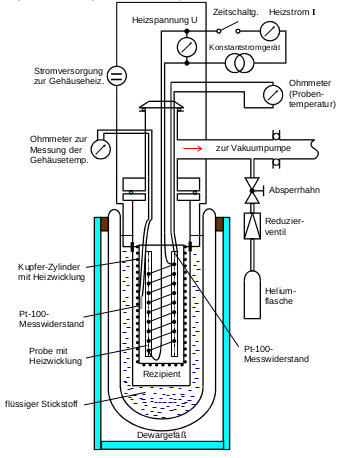
\includegraphics[scale=0.4]{aufbau.png}
  \caption{Der Versuchsaufbau im Schema.}
  \label{fig:1}
\end{figure}
In Abbildung \ref{fig:1} ist die Messapparatur zu sehen. Sie besteht aus dem Rezipienten,
in welchem sich die Probe und ein Kupferzylinder, welcher die Probe umgibt, befinden.
An der Probe und am Zylinder sind Pt-100 Messwiderständen,
deren Widerstand auf Temperaturänderungen reagiert, und Heizwicklungen angebracht.
Außen befindet sich ein Dewargefäß,
in welches der flüssige Stickstoff gefüllt wird, um die Probe und den Zylinder abzukühlen.
Die Temperaturen errechnen sich aus
\begin{equation}
  T = 0.00134 R^2 + 2.296 R - 243.02 \, ,
  \label{widerstand}
\end{equation}
wobei $R$ der Widerstand der Pt-100 Messwiderstände ist.

\subsection{Versuchsdurchführung}
Als erstes wird der Rezipient evakuiert und dann mit Helium gefüllt, um die Probe
ohne gefrierendes Wasser kühlen zu können. Sodann wird flüssiger Stickstoff in das
Dewargefäß gegeben. Sobald die Temperatur auf ca. \SI{80}{\kelvin} gesunken ist,
wird der Rezipient erneut evakuiert und die Probe in \SI{7}{\celsius}-
Schritten erwärmt. Dabei wird die benötigte Zeitdauer, die Temperaturveränderung
von Zylinder und Probe und Heizspannung und -strom aufgenommen. Es wird versucht,
den Zylinder un die Probe auf möglichst der gleichen Temperatur zu halten, damit
keine Wärmestrahlung, Konvektion oder Wärmeleitung auftreten kann. Bei ca. \SI{300}{\kelvin}
wird die Messung gestoppt.
\section{Auswertung}
\subsection{Fehlerrechnung}
Für die Auswertung werden zwei Arten Punktschätzer genutzt. Es gibt:
\begin{equation}
  \overline{T}_\symup{arith.} = \frac{1}{n} \sum_{i=1}^{n} T_{i}
  \label{arith}
\end{equation}
den arithmetischen Mittelwert, sowie:
\begin{equation*}
  \overline{T}_\symup{gew.} = \sum_{i=1}^{n} T_{i}  w_{i}
\end{equation*}
den mit den Gewichten $w_{i}$ gewichteten Mittelwert. Die Summe der Gewichte ist
dabei auf $1$ normiert.
In Fällen, in denen zwei fehlerbehaftete Größen in einer Gleichung zur Bestimmung
einer anderen Größe Verwendung finden, berechnet sich der Gesamtfehler
nach der Gaußschen Fehlerfortpflanzung zu:
\begin{equation*}
    \symup \Delta f(x_1, x_2, ..., x_n) = \sqrt{\left(\frac{\symup df}{\symup dx_1} \symup \Delta
    x_1 \right)^2 +    \left(\frac{\symup df}{\symup dx_2} \symup \Delta
    x_2 \right)^2 + ... + \left(\frac{\symup df}{\symup dx_n} \symup \Delta x_n \right)^2} \ .
\end{equation*}
Für die Fehlerrechnung sowie den mathematischen Teil der Auswertung wird auf $\textsc{Python}$ \cite{python}
zurückgegriffen:\\
Arithmetische Mittelwerte werden durch die Funktion $\textsc{mean}$ aus dem Paket $\textsc{Numpy}$ \cite{numpy}
nach \eqref{arith},
gewichtete Mittelwerte durch manuelles implementieren der jeweiligen Funktion berechnet.
Fehlerfortpflanzung wird
durch die Bibliothek $\textsc{uncertainties}$ \cite{uncertainties} automatisiert.
Regressionen sowie deren Fehler wurden durch die $\textsc{Numpy}$ Funktion $\textsc{polyfit}$
nach einer $\textsc{least-squares}$-Methode mit Polynomen der an den entsprechenden Stellen
angegeben Ordnung durchgeführt. Grafiken wurden mit $\textsc{matplotlib}$ \cite{matplotlib}
erstellt.\\
\\
Widerstände konnten laut Herstellerangaben mit einem relativen Fehler von \SI{0.2}{\percent}
gemessen werden. Für Zeitmessungen wird ein Fehler von $\pm \SI{5}{\second}$ angenommen.

\subsection{Molare Wärmekapazität bei konstantem Druck}
Die molare Wärmekapazität bei konstantem Druck bei konstantem Druck berechnet sich
über die Heizspannung $U$, die Heizstromstärke $I$, die Heizdauer $t_\symup{H}$,
die in $t_\symup{H}$ erreichte Temperaturänderung $\symup{\Delta}T$ sowie über die
Probenmasse $m = \SI{0.342}{\kilo\gram}$ und die Molmasse $M$ des Probenmatials
(für Kupfer: $M = \SI{63.546(3)}{\gram\per\mol}$ \cite{MolKupfer}) nach
\begin{equation}
  c_\symup{p} = \frac{U I t_\symup{H}}{\symup{\Delta}T} \cdot \frac{M}{m}.
  \label{A_eq:1}
\end{equation}
Die nach \eqref{A_eq:1} erhaltenen Werte sind mit den entsprechenden Messwerten
in Tabelle \ref{A_tab:1} zu finden.

\begin{table}[p]
  \centering
  \caption{Übersicht über die Messwerte sowie die daraus bestimmte Größe $c_\symup{p}$}
  \label{A_tab:1}
  \begin{tabular}{c c c c c c c c}
    \toprule
    $T_\symup{Probe, 1}$ / \si{\kelvin} & $T_\symup{Probe, 2}$ / \si{\kelvin} &
    $\symup{\Delta}T$ / \si{\kelvin} & $U$ / \si{\volt} & $I$ / \si{\milli\ampere} &
    $t_\symup{H}$ / \si{\second} & $c_\symup{p}$ / \si{\joule\per\mol\per\kelvin} \\
    \midrule
    79.64  $\pm$ 0.10 & 87.19  $\pm$ 0.12 & 7.54 $\pm$ 0.15 & 15.6 & 149.1 & 240 $\pm$ 5 & 13.75 $\pm$ 0.40 \\
    87.19  $\pm$ 0.12 & 94.05  $\pm$ 0.13 & 6.86 $\pm$ 0.17 & 15.8 & 150.1 & 230 $\pm$ 5 & 14.77 $\pm$ 0.49 \\
    94.28  $\pm$ 0.13 & 101.17 $\pm$ 0.14 & 6.88 $\pm$ 0.19 & 15.8 & 150.3 & 250 $\pm$ 5 & 16.03 $\pm$ 0.56 \\
    101.17 $\pm$ 0.14 & 108.07 $\pm$ 0.16 & 6.91 $\pm$ 0.21 & 15.9 & 150.9 & 260 $\pm$ 5 & 16.78 $\pm$ 0.61 \\
    108.07 $\pm$ 0.16 & 115.24 $\pm$ 0.17 & 7.17 $\pm$ 0.24 & 15.9 & 151.0 & 275 $\pm$ 5 & 17.12 $\pm$ 0.64 \\
    115.24 $\pm$ 0.17 & 122.43 $\pm$ 0.19 & 7.19 $\pm$ 0.26 & 16.0 & 151.5 & 280 $\pm$ 5 & 17.54 $\pm$ 0.70 \\
    122.67 $\pm$ 0.19 & 129.17 $\pm$ 0.20 & 6.49 $\pm$ 0.28 & 17.2 & 163.2 & 230 $\pm$ 5 & 18.47 $\pm$ 0.89 \\
    129.17 $\pm$ 0.20 & 136.16 $\pm$ 0.22 & 7.00 $\pm$ 0.30 & 17.9 & 169.5 & 240 $\pm$ 5 & 19.34 $\pm$ 0.92 \\
    136.16 $\pm$ 0.22 & 143.18 $\pm$ 0.23 & 7.02 $\pm$ 0.32 & 17.6 & 166.8 & 260 $\pm$ 5 & 20.20 $\pm$ 0.99 \\
    143.18 $\pm$ 0.23 & 150.22 $\pm$ 0.25 & 7.04 $\pm$ 0.34 & 17.8 & 168.5 & 250 $\pm$ 5 & 19.78 $\pm$ 1.03 \\
    150.22 $\pm$ 0.25 & 157.05 $\pm$ 0.26 & 6.82 $\pm$ 0.36 & 17.8 & 169.0 & 240 $\pm$ 5 & 19.67 $\pm$ 1.12 \\
    157.29 $\pm$ 0.26 & 164.13 $\pm$ 0.28 & 6.84 $\pm$ 0.38 & 17.9 & 169.0 & 240 $\pm$ 5 & 19.72 $\pm$ 1.17 \\
    164.13 $\pm$ 0.28 & 171.24 $\pm$ 0.29 & 7.11 $\pm$ 0.40 & 17.9 & 169.0 & 240 $\pm$ 5 & 18.98 $\pm$ 1.14 \\
    171.49 $\pm$ 0.29 & 178.13 $\pm$ 0.31 & 6.64 $\pm$ 0.42 & 17.9 & 169.0 & 265 $\pm$ 5 & 22.43 $\pm$ 1.49 \\
    178.13 $\pm$ 0.31 & 185.28 $\pm$ 0.32 & 7.15 $\pm$ 0.44 & 17.8 & 169.0 & 280 $\pm$ 5 & 21.88 $\pm$ 1.41 \\
    185.28 $\pm$ 0.32 & 192.21 $\pm$ 0.34 & 6.93 $\pm$ 0.47 & 17.9 & 169.1 & 275 $\pm$ 5 & 22.33 $\pm$ 1.55 \\
    192.21 $\pm$ 0.34 & 199.16 $\pm$ 0.35 & 6.95 $\pm$ 0.49 & 17.9 & 169.1 & 280 $\pm$ 5 & 22.66 $\pm$ 1.64 \\
    199.16 $\pm$ 0.35 & 206.13 $\pm$ 0.37 & 6.97 $\pm$ 0.51 & 17.9 & 169.1 & 275 $\pm$ 5 & 22.19 $\pm$ 1.67 \\
    206.13 $\pm$ 0.37 & 213.12 $\pm$ 0.38 & 6.99 $\pm$ 0.53 & 17.9 & 169.1 & 290 $\pm$ 5 & 23.33 $\pm$ 1.81 \\
    213.12 $\pm$ 0.38 & 220.13 $\pm$ 0.40 & 7.01 $\pm$ 0.55 & 17.9 & 161.1 & 290 $\pm$ 5 & 22.16 $\pm$ 1.78 \\
    220.13 $\pm$ 0.40 & 227.16 $\pm$ 0.41 & 7.03 $\pm$ 0.57 & 17.9 & 169.2 & 290 $\pm$ 5 & 23.20 $\pm$ 1.93 \\
    227.16 $\pm$ 0.41 & 234.21 $\pm$ 0.43 & 7.05 $\pm$ 0.59 & 17.9 & 169.3 & 300 $\pm$ 5 & 23.95 $\pm$ 2.05 \\
    234.21 $\pm$ 0.43 & 241.29 $\pm$ 0.44 & 7.07 $\pm$ 0.62 & 17.9 & 169.3 & 300 $\pm$ 5 & 23.88 $\pm$ 2.11 \\
    241.29 $\pm$ 0.44 & 248.13 $\pm$ 0.46 & 6.84 $\pm$ 0.64 & 17.9 & 169.3 & 285 $\pm$ 5 & 23.45 $\pm$ 2.22 \\
    248.13 $\pm$ 0.46 & 255.25 $\pm$ 0.47 & 7.12 $\pm$ 0.66 & 17.9 & 169.3 & 290 $\pm$ 5 & 22.95 $\pm$ 2.16 \\
    255.25 $\pm$ 0.47 & 262.13 $\pm$ 0.49 & 6.88 $\pm$ 0.68 & 17.9 & 169.4 & 270 $\pm$ 5 & 22.10 $\pm$ 2.22 \\
    262.13 $\pm$ 0.49 & 269.29 $\pm$ 0.50 & 7.16 $\pm$ 0.70 & 17.9 & 169.4 & 300 $\pm$ 5 & 23.62 $\pm$ 2.35 \\
    269.29 $\pm$ 0.50 & 276.21 $\pm$ 0.52 & 6.92 $\pm$ 0.72 & 17.9 & 169.4 & 300 $\pm$ 5 & 24.42 $\pm$ 2.59 \\
    276.21 $\pm$ 0.52 & 283.15 $\pm$ 0.53 & 6.94 $\pm$ 0.75 & 17.9 & 169.4 & 280 $\pm$ 5 & 22.73 $\pm$ 2.48 \\
    283.15 $\pm$ 0.53 & 290.11 $\pm$ 0.55 & 6.96 $\pm$ 0.77 & 17.9 & 169.4 & 300 $\pm$ 5 & 24.28 $\pm$ 2.71 \\
    290.11 $\pm$ 0.55 & 297.09 $\pm$ 0.57 & 6.98 $\pm$ 0.79 & 17.9 & 169.4 & 295 $\pm$ 5 & 23.81 $\pm$ 2.72 \\
    \bottomrule
  \end{tabular}
\end{table}

\subsection{Molare Wärmekapazität bei konstantem Volumen}
Die molare Wärmekapazität bei konstantem Volumen $c_\symup{V}$ kann aus $c_\symup{p}$
über die Korrekturformel
\begin{equation}
  c_\symup{V} = c_\symup{p} - 9 \alpha^2 \kappa V_0 T
  \label{A_eq:2}
\end{equation}
bestimmt werden. $\alpha$ bezeichnet dabei den temperaturabhängigen linearen
Ausdehnungskoeffizienten, $\kappa$ das Kompressionsmodul (für Kupfer: $\kappa =
\SI{137.8}{\giga\pascal}$ \cite{KupferKappa}), $V_0$ das Molvolumen
(für Kupfer: $V_0 = \SI{7.10}{\centi\metre\cubed\per\mol}$ \cite{MolKupfer})
und $T$ die Temperatur. Als Temperatur wird der Mittelwert zwischen Start- und
Endpunkt jeder Messung genommen. Zur Bestimmung von $\alpha$ werden die gegebenen
Werte \cite[S. 5, Tabelle 2]{anleitung} eingelesen und mit einem Polynom 4. Grades gefittet. Es ergeben sich die
folgenden Koeffizienten:
\begin{align*}
    a_4 &= \SI{-8.16(75)e-15}{\per\kelvin\tothe{5}}\\
    a_3 &= \SI{7.39(55)e-12}{\per\kelvin\tothe{4}}\\
    a_2 &= \SI{-2.53(14)e-09}{\per\kelvin\cubed}\\
    a_1 &= \SI{4.07(16)e-07}{\per\kelvin\squared}\\
    a_0 &= \SI{-1.13(6)e-05}{\per\kelvin}.
\end{align*}
Eine graphische Darstellung der Regression findet sich in Abbildung \ref{A_abb:1}. Die nach \eqref{A_eq:2}
bestimmten $c_\symup{V}$-Werte sind in Tabelle \ref{A_tab:2} zu finden. Eine grafische Darstellung
der $c_\symup{p}$- und $c_\symup{V}$-Werte findet sich in \ref{A_abb:2}.

\begin{figure}[h!]
  \centering
  \subcaptionbox{Fit des linearen Ausdehnungskoeffizienten. \label{A_abb:1}}[0.48\textwidth]{
  \centering
  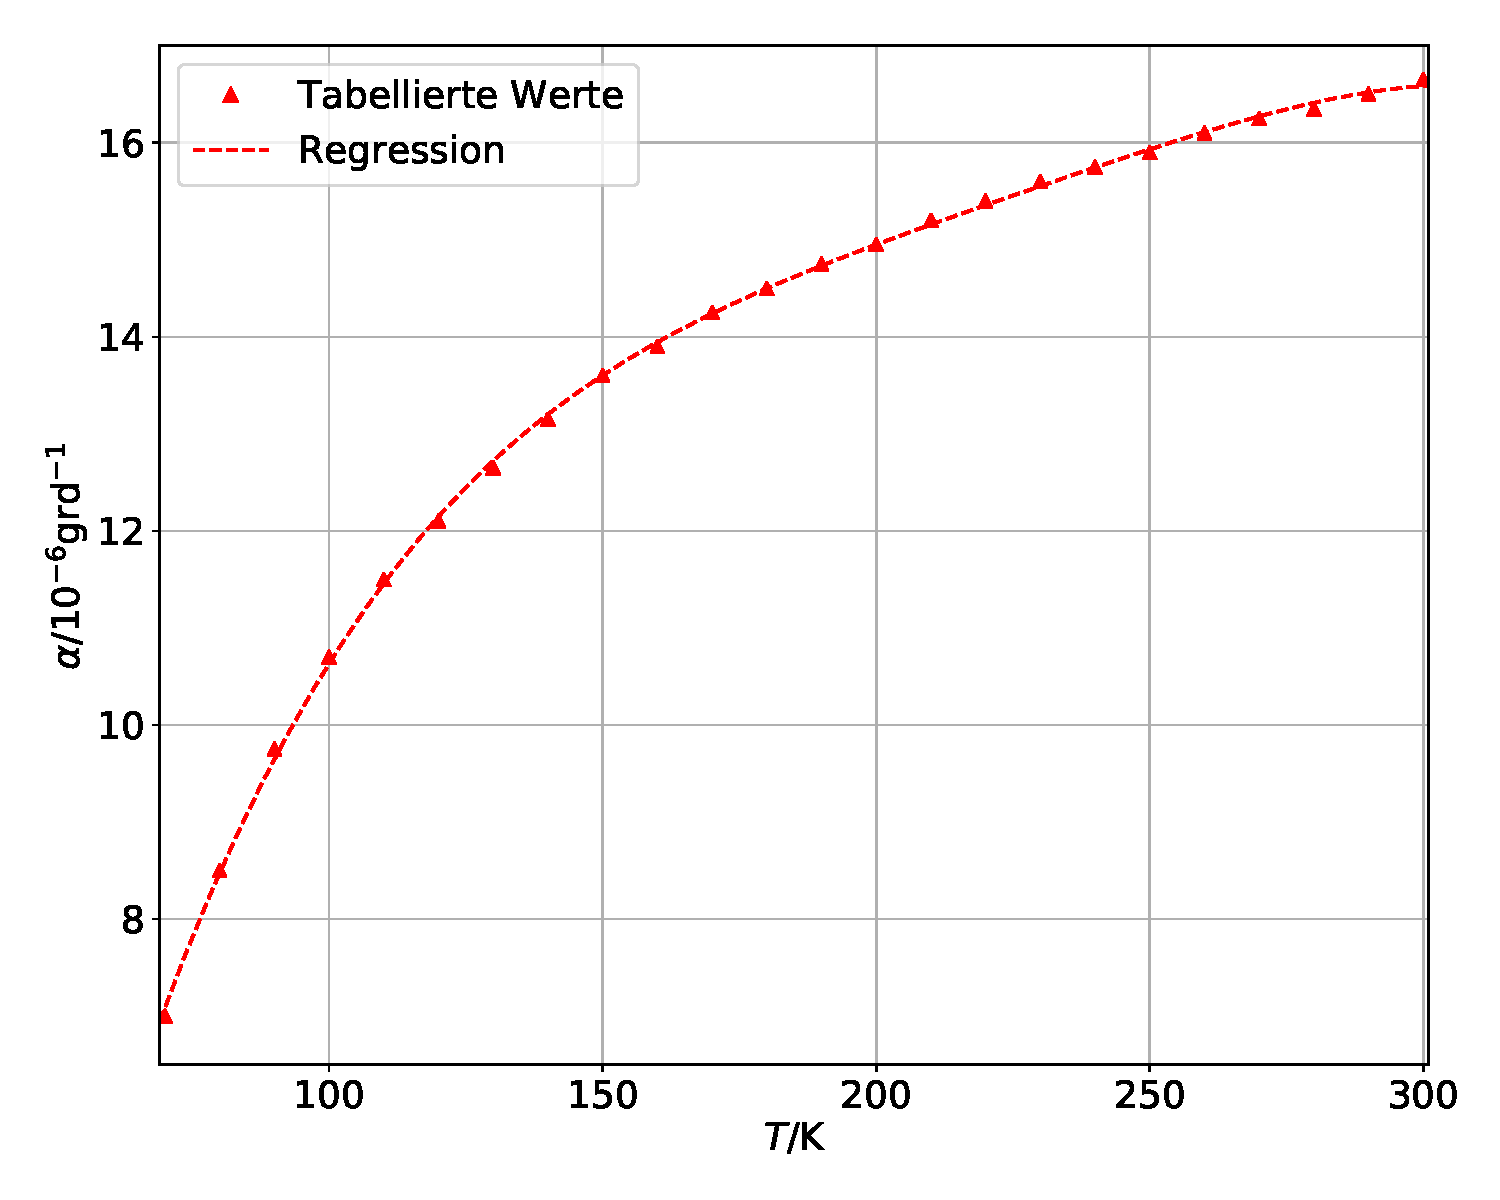
\includegraphics[width=0.48\textwidth]{Koeff.pdf}
  }
  \subcaptionbox{Verlauf der $c_\symup{p}$- und $c_\symup{V}$-Werte. \label{A_abb:2}}[0.48\textwidth]{
  \centering
  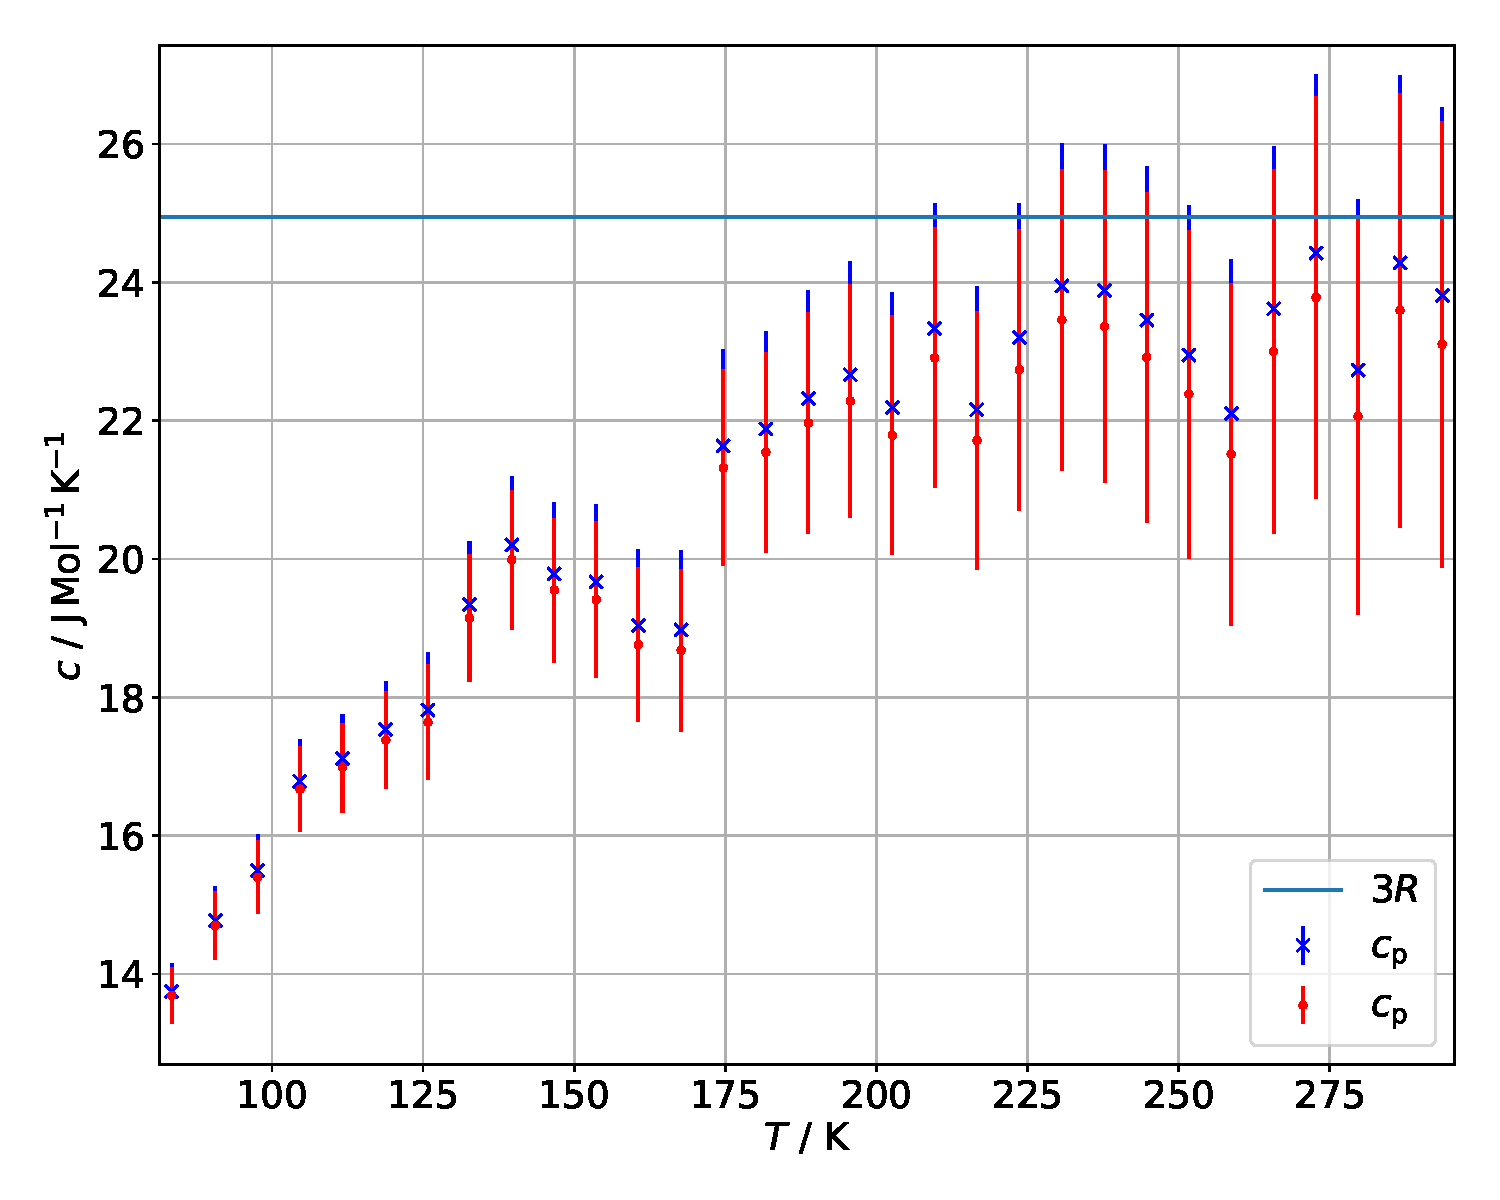
\includegraphics[width=0.48\textwidth]{Kapaz.pdf}
  }
  \label{A_Abb:3}
  \caption{ }
\end{figure}

\begin{table}[p]
  \centering
  \caption{Übersicht über die für die Rechnung notwendigen Größen sowie die
          daraus bestimmten Werte für $c_\symup{V}$. Werte bis \SI{170}{\kelvin}
          sind durch eine Linie abgetrennt.}
  \label{A_tab:2}
  \begin{tabular}{c c c c}
    \toprule
    $\overline{T}$ / \si{\kelvin} & $\alpha_\symup{\overline{T}}$ /
    \SI{e-6}{\per\kelvin} & $c_\symup{p}$ / \si{\joule\per\mol\per\kelvin}
    & $c_\symup{V}$ / \si{\joule\per\mol\per\kelvin}\\
    \midrule
    83.41  $\pm$ 0.08 & 8.90  $\pm$ 1.82  & 13.75 $\pm$ 0.40 & 13.69 $\pm$ 0.40 \\
    90.62  $\pm$ 0.09 & 9.71  $\pm$ 2.03  & 14.77 $\pm$ 0.49 & 14.70 $\pm$ 0.49 \\
    97.73  $\pm$ 0.10 & 10.43 $\pm$ 2.25  & 16.03 $\pm$ 0.56 & 15.93 $\pm$ 0.56 \\
    104.62 $\pm$ 0.11 & 11.03 $\pm$ 2.49  & 16.78 $\pm$ 0.61 & 16.67 $\pm$ 0.62 \\
    111.66 $\pm$ 0.12 & 11.58 $\pm$ 2.75  & 17.12 $\pm$ 0.64 & 16.98 $\pm$ 0.65 \\
    118.84 $\pm$ 0.13 & 12.07 $\pm$ 3.03  & 17.54 $\pm$ 0.70 & 17.38 $\pm$ 0.70 \\
    125.92 $\pm$ 0.14 & 12.50 $\pm$ 3.34  & 18.47 $\pm$ 0.89 & 18.30 $\pm$ 0.89 \\
    132.67 $\pm$ 0.15 & 12.86 $\pm$ 3.65  & 19.34 $\pm$ 0.92 & 19.14 $\pm$ 0.92 \\
    139.67 $\pm$ 0.16 & 13.19 $\pm$ 3.99  & 20.20 $\pm$ 0.99 & 19.99 $\pm$ 1.00 \\
    146.70 $\pm$ 0.17 & 13.48 $\pm$ 4.36  & 19.78 $\pm$ 1.03 & 19.55 $\pm$ 1.04 \\
    153.64 $\pm$ 0.18 & 13.73 $\pm$ 4.76  & 19.67 $\pm$ 1.12 & 19.41 $\pm$ 1.13 \\
    160.71 $\pm$ 0.19 & 13.97 $\pm$ 5.18  & 19.72 $\pm$ 1.17 & 19.44 $\pm$ 1.19 \\
    167.69 $\pm$ 0.20 & 14.17 $\pm$ 5.63  & 18.98 $\pm$ 1.14 & 18.68 $\pm$ 1.17 \\
    \midrule
    174.81 $\pm$ 0.21 & 14.37 $\pm$ 6.12  & 22.43 $\pm$ 1.49 & 22.12 $\pm$ 1.52 \\
    181.70 $\pm$ 0.22 & 14.54 $\pm$ 6.63  & 21.88 $\pm$ 1.41 & 21.54 $\pm$ 1.45 \\
    188.74 $\pm$ 0.23 & 14.70 $\pm$ 7.18  & 22.33 $\pm$ 1.55 & 21.97 $\pm$ 1.59 \\
    195.68 $\pm$ 0.24 & 14.86 $\pm$ 7.75  & 22.66 $\pm$ 1.64 & 22.28 $\pm$ 1.69 \\
    202.64 $\pm$ 0.25 & 15.01 $\pm$ 8.36  & 22.19 $\pm$ 1.67 & 21.79 $\pm$ 1.73 \\
    209.62 $\pm$ 0.26 & 15.15 $\pm$ 9.01  & 23.33 $\pm$ 1.81 & 22.91 $\pm$ 1.88 \\
    216.62 $\pm$ 0.28 & 15.29 $\pm$ 9.70  & 22.16 $\pm$ 1.78 & 21.71 $\pm$ 1.87 \\
    223.64 $\pm$ 0.29 & 15.43 $\pm$ 10.43 & 23.20 $\pm$ 1.93 & 22.74 $\pm$ 2.03 \\
    230.69 $\pm$ 0.30 & 15.57 $\pm$ 11.20 & 23.95 $\pm$ 2.05 & 23.46 $\pm$ 2.17 \\
    237.75 $\pm$ 0.31 & 15.70 $\pm$ 12.02 & 23.88 $\pm$ 2.11 & 23.36 $\pm$ 2.26 \\
    244.71 $\pm$ 0.32 & 15.83 $\pm$ 12.87 & 23.45 $\pm$ 2.22 & 22.91 $\pm$ 2.39 \\
    251.69 $\pm$ 0.33 & 15.96 $\pm$ 13.77 & 22.95 $\pm$ 2.16 & 22.38 $\pm$ 2.37 \\
    258.69 $\pm$ 0.34 & 16.09 $\pm$ 14.72 & 22.10 $\pm$ 2.22 & 21.52 $\pm$ 2.47 \\
    265.71 $\pm$ 0.35 & 16.20 $\pm$ 15.72 & 23.62 $\pm$ 2.35 & 23.00 $\pm$ 2.63 \\
    272.75 $\pm$ 0.36 & 16.31 $\pm$ 16.77 & 24.42 $\pm$ 2.59 & 23.78 $\pm$ 2.90 \\
    279.68 $\pm$ 0.37 & 16.41 $\pm$ 17.86 & 22.73 $\pm$ 2.48 & 22.06 $\pm$ 2.87 \\
    286.63 $\pm$ 0.38 & 16.49 $\pm$ 19.01 & 24.28 $\pm$ 2.71 & 23.60 $\pm$ 3.14 \\
    293.60 $\pm$ 0.39 & 16.55 $\pm$ 20.22 & 23.81 $\pm$ 2.72 & 23.10 $\pm$ 3.23 \\
    \bottomrule
  \end{tabular}
\end{table}

\subsection{Bestimmend der Debey-Temperatur}
Zur Bestimmung der $\textsc{Debeye}$-Temperatur werden zuerst die der gegebenen Tabelle \cite[S. 5, Tabelle 1]{anleitung}
entnommennen Werte für $\theta_D/T$ in dem auf die bis \SI{170}{\kelvin} passenden
Bereich (\numrange[range-phrase = --]{13.305}{20.205}) mit einem Polynom
1. Ordnung gefittet. Es ergeben sich folgende Koeffizienten:
\begin{align*}
  a_0 &= \SI{7.043}{\mol\kelvin\per\joule} \\
  a_1 &= \SI{-0.244}{\mol\squared\kelvin\squared\per\joule\squared}
\end{align*}
Die Fehler treten dabei erst in der 13. Mantisse auf und werden daher hier nicht
dargestellt, in den automatisierten Rechnungen aber weiterhin beachtet. Der Fit ist
in Abbildung \ref{A_abb:4} dargestellt. Die Werte für $\theta_D/T$ werden nun durch
Auswerten der Fit-Funktion an den entsprechenden $c_\symup{V}$-Werten bestimmt.
Die so bestimmten $\theta_D/T$-Werte werden mit dem entsprechenden $\overline{T}$
multipliziert, um die $\textsc{Debeye}$-Temperaturen $\theta_D$ zu bestimmen.
Die resultierenden Werte sind in Tabelle \ref{A_tab:3} eingetragen.
Mittelwertbildung wie eingangs beschrieben liefert folgende Werte:
\begin{align*}
  \theta_{D, arrith.} &= \SI{331(9)}{\kelvin} \\
  \theta_{D, gew.} &= \SI{330(9)}{\kelvin}.
\end{align*}
Als Gewichte wurde dabei das Verhältnis zwischen Proben- und Zylindertemperatur
so gewählt, dass Messwerte mit stark unterschiedlichen Temperataturen weniger
stark gewichtet sind. Die Gewichte wurden in der Summe auf \num{1} normiert.

\begin{figure}[h!]
  \centering
  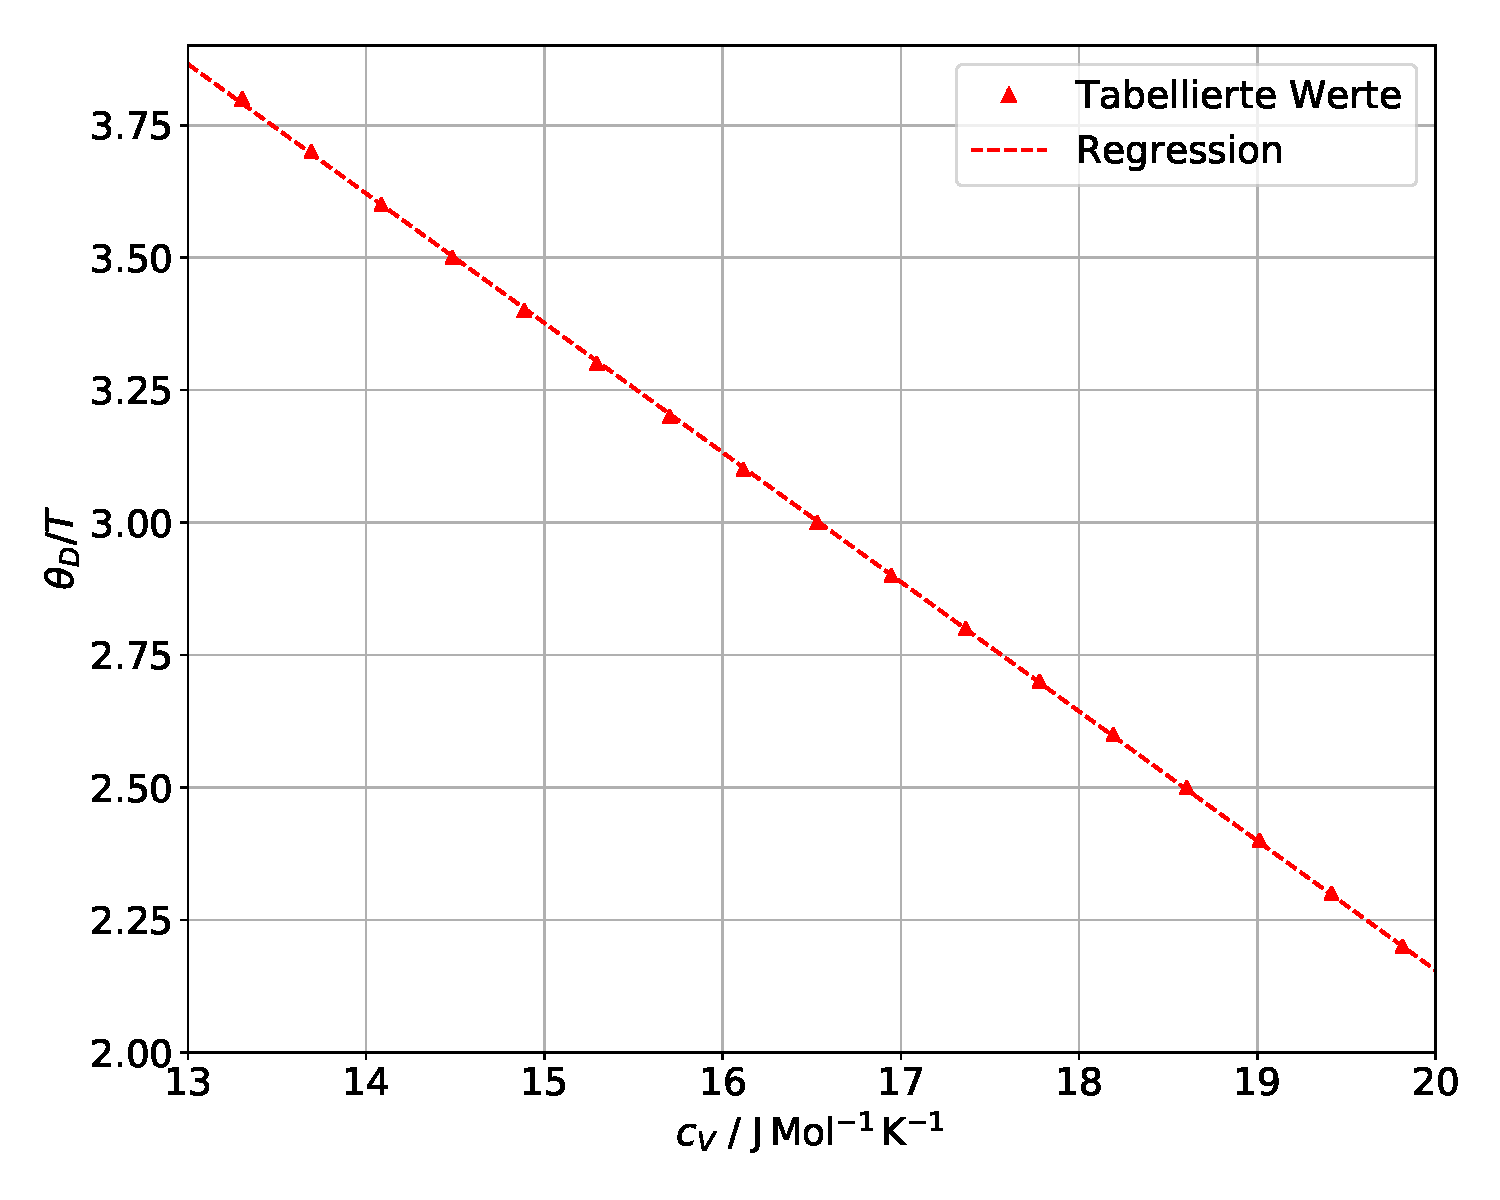
\includegraphics[scale=0.4]{Debeye.pdf}
  \caption{Fit der Debeye-Funktion.}
  \label{A_abb:4}
\end{figure}

\begin{sidewaystable}[p]
  \centering
  \caption{Übersicht über die für die Rechnung notwendigen Größen sowie die
          daraus bestimmten Werte für $\theta_D$. Es sind weiterhin die für
          die spätere Berechnung des gewichteten Mittelwertes notwendigen Werte
          eingetragen.}
  \label{A_tab:3}
  \begin{tabular}{c c c c c c c}
    \toprule
    $\overline{T}$ / \si{\kelvin}
    & $T_\symup{zyl., 1}$ / \si{\kelvin}
    & $T_\symup{zyl., 2}$ / \si{\kelvin}
    & $\overline{T}_\symup{zyl.}$ / \si{\kelvin}
    & $\overline{T}/\overline{T}_\symup{zyl.}$
    & $c_\symup{V}$ / \si{\joule\per\mol\per\kelvin}
    & $\theta_D$ / \si{\kelvin}\\
    \midrule
    83.41  $\pm$ 0.08 & 80.82  $\pm$ 0.10 & 88.13  $\pm$ 0.12 & 84.48  $\pm$ 0.08 & 98.74  $\pm$ 0.13 & 13.69 $\pm$ 0.40 & 308.34 $\pm$ 8.20 \\
    90.62  $\pm$ 0.09 & 88.13  $\pm$ 0.12 & 94.52  $\pm$ 0.13 & 91.33  $\pm$ 0.09 & 99.22  $\pm$ 0.13 & 14.70 $\pm$ 0.49 & 312.66 $\pm$ 10.98 \\
    97.73  $\pm$ 0.10 & 94.76  $\pm$ 0.13 & 100.69 $\pm$ 0.14 & 97.72  $\pm$ 0.10 & 100.00 $\pm$ 0.14 & 15.93 $\pm$ 0.56 & 307.73 $\pm$ 13.32 \\
    104.62 $\pm$ 0.11 & 100.93 $\pm$ 0.14 & 109.03 $\pm$ 0.16 & 104.98 $\pm$ 0.11 & 99.66  $\pm$ 0.14 & 16.67 $\pm$ 0.62 & 310.53 $\pm$ 15.77 \\
    111.66 $\pm$ 0.12 & 109.50 $\pm$ 0.16 & 115.96 $\pm$ 0.18 & 112.73 $\pm$ 0.12 & 99.05  $\pm$ 0.15 & 16.98 $\pm$ 0.65 & 322.92 $\pm$ 17.65 \\
    118.84 $\pm$ 0.13 & 115.96 $\pm$ 0.18 & 122.67 $\pm$ 0.19 & 119.32 $\pm$ 0.13 & 99.60  $\pm$ 0.15 & 17.38 $\pm$ 0.70 & 332.09 $\pm$ 20.47 \\
    125.92 $\pm$ 0.14 & 123.39 $\pm$ 0.19 & 129.41 $\pm$ 0.20 & 126.40 $\pm$ 0.14 & 99.62  $\pm$ 0.16 & 18.30 $\pm$ 0.89 & 323.68 $\pm$ 27.42 \\
    132.67 $\pm$ 0.15 & 129.89 $\pm$ 0.20 & 137.13 $\pm$ 0.22 & 133.51 $\pm$ 0.15 & 99.37  $\pm$ 0.16 & 19.14 $\pm$ 0.92 & 313.62 $\pm$ 29.91 \\
    139.67 $\pm$ 0.16 & 137.61 $\pm$ 0.22 & 142.46 $\pm$ 0.23 & 140.03 $\pm$ 0.16 & 99.74  $\pm$ 0.16 & 19.99 $\pm$ 1.00 & 301.30 $\pm$ 34.27 \\
    146.70 $\pm$ 0.17 & 142.94 $\pm$ 0.23 & 155.58 $\pm$ 0.26 & 149.26 $\pm$ 0.17 & 98.29  $\pm$ 0.16 & 19.55 $\pm$ 1.04 & 332.25 $\pm$ 37.41 \\
    153.64 $\pm$ 0.18 & 155.58 $\pm$ 0.26 & 166.34 $\pm$ 0.28 & 160.96 $\pm$ 0.19 & 95.45  $\pm$ 0.16 & 19.41 $\pm$ 1.13 & 353.10 $\pm$ 42.43 \\
    160.71 $\pm$ 0.19 & 166.58 $\pm$ 0.28 & 173.21 $\pm$ 0.30 & 169.89 $\pm$ 0.20 & 94.60  $\pm$ 0.16 & 19.44 $\pm$ 1.19 & 368.31 $\pm$ 46.76 \\
    167.69 $\pm$ 0.20 & 173.45 $\pm$ 0.30 & 176.89 $\pm$ 0.30 & 175.17 $\pm$ 0.21 & 95.73  $\pm$ 0.16 & 18.68 $\pm$ 1.17 & 415.43 $\pm$ 47.88 \\
    \bottomrule
  \end{tabular}
\end{sidewaystable}

\subsection{Bestimmen eines Referenzwertes für Debey-Frequenz und Temperatur}
Nach \eqref{fürrune<3} folgt mit
\begin{align*}
  N_L &= N_\symup{A} \frac{m}{M} = \num{3.24107e24} \\
  L &= \sqrt[3]{V_0 \frac{m}{M}} = \SI{33.682}{\milli\metre} \\
  v_{\symup{long}} &= \SI{4.7}{\kilo\metre\per\second}\\
  v_{\symup{trans}} &= \SI{2.26}{\kilo\metre\per\second}
\end{align*}
für $\omega_D$ ein Wert von
\begin{equation*}
  \omega_D = \SI{43.5}{\tera\hertz}.
\end{equation*}
Weiter folgt:
\begin{equation*}
  \theta_D = \frac{\hbar\omega_D}{k} = \SI{332.36}{\kelvin}.
\end{equation*}

\section{Diskusion}
Bei Betrachten der $c_\symup{p}$- und $c_\symup{V}$-Werte zeigt sich im weitesten
der zu erwartende Verlauf (siehe Grafik \ref{A_abb:2}). Insbesondere ist die
asymptotische Annäherung an den Wert $3R$ zu erahnen. Lediglich das
Tieftemperaturverhalten kann nicht abgebildet werden. Auch der Vergleich
zwischen den aus den Messwerten bestimmten Werten für $\theta_D$ sowie dem
bestimmten Referenzwert lässt auf eine gute Messung schließen. Hier konnten die
Messwerte den Referenzwert im Rahmen der Messungenauigkeit treffen.\\
Als Problematisch gestaltete sich das gleichmäßige temperieren von Probe und
Zylinder, was prinzipell als systematischer Fehler zu betrachten ist. Die geringen
Abweichungen der nominellen Werte des gewichteten und arrithmetischen Mittelwertes
zeigen aber, dass der Einfluss hier nur gering ist. Die Aussagekraft dieser Werte
ist jedoch begrenzt, da pro Heizperiode nur der Mittelwert der Temperaturen
betrachtet wurde. An dieser Stelle bietet sich eine digitale Datenaufnahme an, mit der ein
zeitlich genauer aufgelöster Temperaturverlauf erzeugt werden könnte. Durch ein
herunterkühlen des Versuchsaufbaus auf tiefere Temperaturen als die von flüssigem
Stickstoff könnte weiter ermöglicht werden, den Tieftemperaturverlauf abzubilden.

\newpage
\nocite{*}
\printbibliography
